\scanpage{41}

datum of the commutativities $\alpha_{D^*U}$, and write the compatibility conditions with $\alpha,\alpha'$ and $k,k'$. The datum of $\alpha_{D^*,U}$ is equivalent to that of systems of elements
\[
\boxed{\beta_{i'}\in\mathcal E'}\qquad(i'\in I')
\]
\deleted{\illegible{1}}\inserted{such that} one has, in the diagrams
\diagram{\begin{tikzcd}[ampersand replacement=\&]
G'_{i'} \arrow[r,"\rho'_{i'}"] \arrow[d,"f_{i'}"'] \& \mathcal E' \arrow[d,"f_{\mathcal E}"] \\
G_{\tau i'} \arrow[r,"\rho_{\tau i'}"'] \& \mathcal E
\end{tikzcd}}
the relation
\[
f_{\mathcal E}\rho'_{i'}=\operatorname{int}(\beta_{i'})\rho_{\tau i'}\circ f_{i'}.
\]

It remains to express the \inserted{two} compatibilities \deleted{with} of
$(\unsure{f_{D^*}},f_D,f_U,\unsure{\alpha_{D^*D}},\alpha_{De},\alpha_{D^*U},\alpha_{Ue})$ with
itself and with $K$ --- the second compatibility is simply the compatibility of the $f_{i'}$ with the $k'_{i'},k_i$, i.e.
\[
f_{i'}\circ k'_{i'}=k_i\qquad(i=\tau i')
\]
and the first \uline{unless I am mistaken} is expressed by the ``commutativity''
\[
\deleted{\unsure{\rho(\beta_{i'})|p(\beta_{i'})}}\alpha\gamma'_{i'}
 =\inserted{\unsure{\rho(\beta_{i'})|p(\beta_{i'})}}\gamma_i\alpha_{i'}
 \qquad\forall i'\in I'
\]
\[
\boxed{\alpha_{i'}=\gamma_i^{-1}\unsure{\rho|p}(\beta_{i'}^{-1})\alpha\gamma'_{i'}}
\]
\margin{40}

\scanpage{42}
\mspage{19}

In summary, the \unsure{homomorphisms}, into a \inserted{system of} \deleted{\illegible{1}} commutative diagrams
\diagram{\begin{tikzcd}[ampersand replacement=\&, column sep=small]
1 \arrow[r] \& T(\bar K) \arrow[r,"k_i"] \arrow[dr] \& \mathcal E_i \arrow[r,"p_i"] \arrow[dr,"\rho_i"] \& \Gamma \arrow[dr,"\operatorname{int}(\gamma_i)"] \& \\
\& 1 \arrow[r] \& \pi \arrow[r] \& \mathcal E \arrow[r,"p"'] \& \Gamma
\end{tikzcd}\qquad$(i\in I)$}
from an analogous system, relative to a set of indices $I'$, is given by a map
\[
\tau:I'\longrightarrow I
\]
and for every $i'\in I'$, setting $i=\tau(i')$, of a system of vertical arrows $f_{i'}\inserted{{}:\mathcal E'_{i'}\longrightarrow\mathcal E_i}$, and of a \inserted{vertical} arrow $f_{\mathcal E}:\mathcal E'\longrightarrow\mathcal E$, finally \deleted{of systems} \deleted{$\alpha\in\Gamma$ and} of a system of elements $\beta_{i'}\in\mathcal E$ and of an $\alpha\in\Gamma$, \deleted{satisfying} fitting into the system of diagrams
\diagram{\begin{tikzcd}[ampersand replacement=\&,column sep=1.3em,row sep=2.2em]
1\arrow[rr] \& \& T(\bar K)\arrow[rr,"k'_{i'}"]\arrow[dr,"\varepsilon'_{i'}"']\arrow[dd,"d_{i'}"'] \& \& \mathcal E'_{i'}\arrow[rr,"p'_{i'}"]\arrow[dr,hook,"\rho'_{i'}"]\arrow[dd,"f_{i'}"' near start] \& \& \Gamma\arrow[dr,"\operatorname{int}(\gamma'_{i'})"]\arrow[dd,"\operatorname{int}(\alpha_{i'})"' near start] \& \\
\& 1\arrow[rr] \& \& \pi'\arrow[rr]\arrow[dd] \& \& \mathcal E'\arrow[rr,"p'"]\arrow[dd,"f_{\mathcal E}" near start] \& \& \Gamma\arrow[dd,"\operatorname{int}(\alpha)"] \\
1\arrow[rr] \& \& T(\bar K)\arrow[rr,"k_i"]\arrow[dr,"\varepsilon_i"'] \& \& \mathcal E_i\arrow[rr,"p_i"]\arrow[dr,hook,"\rho_i"'] \& \& \Gamma\arrow[dr,"\operatorname{int}(\gamma_i)"] \& \\
\& 1\arrow[rr] \& \& \pi\arrow[rr] \& \& \mathcal E\arrow[rr,"p"'] \& \& \Gamma
\end{tikzcd}
[Prism: the second and fourth rows are shifted to the right. The vertical arrow $d_{i'}$ between the two $T(\bar K)$ is drawn with a double stroke; $\pi'\longrightarrow\pi$ without a label. Below the arrow $p_i$, near the tip of $\rho_i$, $\unsure{\beta_{i'}}$ overwritten; farther along the same arrow, near the tip toward $\Gamma$, an overwritten sign \illegible{1}.]}

\margin{\uline{N.B.} Since the $\mathcal E_i\hookrightarrow\mathcal E$ are injective, \deleted{the} $f_{i'}$ is known when one knows $f_{\mathcal E}$ and $\beta_{i'}$ (the existence \unsure{of|of the} $f_{i'}$ is therefore a condition on the pairs $f_{\mathcal E},\beta_{i'}$ \illegible{1} \unsure{namely} that $\operatorname{int}(\beta_{i'})^{-1}f_{\mathcal E}\rho'_{i'}$ \unsure{$\mathcal E'_{i'}$} into $\unsure{\rho_i(\mathcal E_i)|p_i(\mathcal E_i)}$)}

\margin{\uline{N.B.} We may assume the $\gamma'_{i'},\gamma_i$ equal to $1$ (by choosing the image of $\unsure{\psi|\varphi}\sigma(D_i^*)$ \unsure{over} $\operatorname{Spec}(\bar K)$ via the isomorphism of $\varphi(\rho(D_i^*))\simeq\varphi(\unsure{\widetilde U|\widetilde U_i})$ \unsure{with} $\operatorname{Spec}\bar K$}

\unsure{where we have} set
\[
(*)\quad\alpha_{i'}=\gamma_i^{-1}p(\beta_{i'}^{-1})\alpha\gamma'_{i'}
\qquad\text{i.e.}\quad\deleted{\illegible{1}}\ \alpha\gamma'_{i'}=p(\beta_{i'})\gamma_i\alpha_{i'}
\]
and \unsure{i.e.|where} the rear \inserted{vertical} face of the prisms is commutative (two conditions, on two squares), the front \inserted{vertical} face too (this is \uline{one} condition, on the right-hand square, the other square
\margin{41}

\scanpage{43}

being commutative follows from this by definition of $\pi'\longrightarrow\pi$ as induced by $f_{\mathcal E}\ldots$), the left vertical face of the right-hand cube being commutative modulo the commutativity isomorphism $\operatorname{int}(\beta_{i'})$, and the right vertical face being \deleted{\unsure{cont}}commutative (not only, by the preceding condition, on
\[
\unsure{\Gamma'_{i'}}=\operatorname{Im}(\mathcal E'_{i'}\xrightarrow{p'_{i'}}\Gamma),
\]
but on the whole of $\Gamma$) by virtue of the more precise relation $(*)$.

\figure{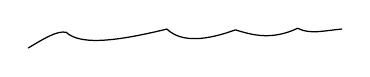
\begin{tikzpicture}[x=1cm,y=1cm,line cap=round,line join=round]
\draw[line width=0.45pt] (0,0) .. controls (0.20,0.12) and (0.36,0.22) .. (0.48,0.20)
.. controls (0.67,0.02) and (1.18,0.10) .. (1.76,0.24)
.. controls (1.95,0.06) and (2.27,0.10) .. (2.63,0.23)
.. controls (2.83,0.17) and (3.08,0.09) .. (3.42,0.25)
.. controls (3.58,0.17) and (3.75,0.22) .. (3.98,0.24);
\end{tikzpicture}}

Messy category made precise (corresponding to a $\Pi_U$ that is \uline{connected}):

These objects are the \deleted{pairs $(I$, \unsure{systems}}\inserted{homomorphisms of groups} that are profinite \deleted{(\unsure{indexed} by a finite set $I$) of the homomorphism}
\[
\mathcal E\xrightarrow{p}\Gamma
\]
(giving rise to an exact sequence:
\[
1\longrightarrow\pi\xrightarrow{\unsure{k|\kappa}}\mathcal E\xrightarrow{p}\Gamma
\]
)
and a \inserted{finite} set of subgroups (indexed by a set $I$ of indices)
\[
\mathcal E_i\overset{\rho_i}{\lhook\joinrel\longrightarrow}\mathcal E,
\]
and of isomorphisms
\[
\mathcal E_i\cap\pi\overset{k_i}{\simeq}T(\bar K)
\]
\margin{42}

\scanpage{44}
\mspage{20}

A homomorphism from a system
$(\mathcal E',p',(\mathcal E'_{i'})_{i'\in I'},(k'_{i'})_{i'\in I'})$
into a system
$(\mathcal E,p,(\mathcal E_i)_{i\in I},(k_i)_{i\in I})$
is given by by a homomorphism
\[
f:\mathcal E'\longrightarrow\mathcal E
\]
\[
\beta_{i'}\in\mathcal E\quad(i'\in I'),\qquad\alpha\in\Gamma,
\]
such that one has the conditions:

\figure{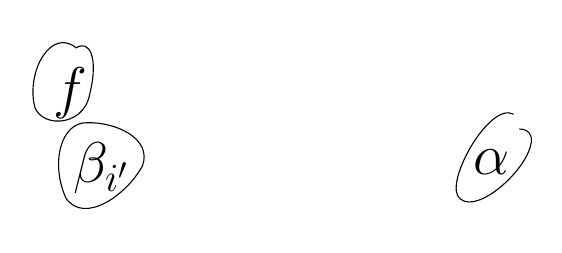
\begin{tikzpicture}[x=1cm,y=1cm,line cap=round,line join=round]
\begin{scope}[yshift=-0.35cm]
\node[font=\fontsize{22}{24}\selectfont] at (0,1.30) {$f$};
\draw (0.08,1.88) .. controls (-0.22,2.13) and (-0.53,1.64) .. (-0.46,1.19)
.. controls (-0.43,0.86) and (0.17,0.85) .. (0.25,1.29)
.. controls (0.37,1.77) and (0.24,1.99) .. (0.08,1.88);
\end{scope}
\node[font=\fontsize{22}{24}\selectfont] at (0.40,0) {$\beta_{i'}$};
\draw (0.22,0.58) .. controls (-0.12,0.59) and (-0.25,0.06) .. (-0.05,-0.38)
.. controls (0.18,-0.71) and (0.71,-0.35) .. (0.92,0.03)
.. controls (1.05,0.38) and (0.58,0.59) .. (0.22,0.58);
\node[font=\fontsize{22}{24}\selectfont] at (5.35,0.08) {$\alpha$};
\draw (5.63,0.69) .. controls (5.32,0.85) and (4.72,-0.23) .. (4.96,-0.39)
.. controls (5.18,-0.57) and (5.77,-0.05) .. (5.85,0.29)
.. controls (5.89,0.42) and (5.82,0.50) .. (5.71,0.50);
\end{tikzpicture}}

\margin{The $\beta_{i'}$ not unique (if $\beta_{i'}$ works, also $\gamma\beta_{i'}$, with $\unsure{\gamma|\gamma_i}\in\operatorname{Im}k_i$). But $\alpha$ unique \unsure{?!|??}}

$1^\circ)$\quad $p\circ f_{\mathcal E}=\operatorname{int}(\alpha)\,p'$

$2^\circ)$\quad $\forall i'\in I',\quad\exists i\in I$ (unique!) such that
\[
\operatorname{int}(\beta_{i'}^{-1})f(\mathcal E'_{i'})\subset\mathcal E_i
\]
and an integer $d_{i'}\in\mathbb N^*$ such that
\[
\operatorname{int}(\beta_{i'}^{-1})f\,k'_{i'}
 =k_i\circ(d_{i'}\cdot\operatorname{id}_{T(\bar K)})
\]

\margin{N.B.: $d_{i'}$ is also unique\ldots}

\margin{[thus $\operatorname{int}(\beta_{i'}^{-1})\overbrace{\unsure{\operatorname{Im}(fk'_{i'})|\operatorname{Im}k'_{i'}}}^{L'_{i'}}\subset\underbrace{\operatorname{Im}k_i}_{L_i}$ and \unsure{even} \deleted{\unsure{this} image} $\operatorname{int}(\beta_{i'}^{-1})\unsure{L'_{i'}}=d_{i'}L_i$.]}

\figure{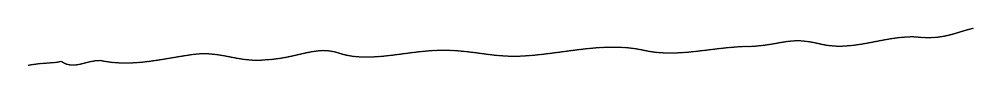
\begin{tikzpicture}[x=1cm,y=1cm,line cap=round,line join=round]
\draw[line width=0.45pt] (0,0) .. controls (0.22,0.04) and (0.30,0.02) .. (0.42,0.05)
.. controls (0.58,-0.07) and (0.73,0.07) .. (0.92,0.06)
.. controls (1.30,-0.02) and (1.64,0.07) .. (2.04,0.13)
.. controls (2.44,0.20) and (2.64,0.03) .. (3.02,0.07)
.. controls (3.43,0.09) and (3.66,0.26) .. (3.96,0.15)
.. controls (4.37,0.02) and (4.86,0.21) .. (5.35,0.19)
.. controls (5.79,0.17) and (5.95,0.08) .. (6.44,0.13)
.. controls (6.94,0.18) and (7.37,0.29) .. (7.82,0.19)
.. controls (8.26,0.09) and (8.70,0.24) .. (9.18,0.24)
.. controls (9.58,0.26) and (9.66,0.37) .. (10.06,0.27)
.. controls (10.48,0.17) and (10.87,0.38) .. (11.28,0.36)
.. controls (11.62,0.32) and (11.78,0.42) .. (12.00,0.47);
\end{tikzpicture}}

I realize that it is better to replace the $\beta_{i'}$ by the $\beta_{i'}^{-1}$, i.e. to take the commutation isomorphism rather in the direction
\[
f_{\mathcal E}\rho'_{i'}\xrightarrow{\beta_{i'}}\rho_i f_{i'}
\]
than in the opposite direction. Moreover, conceptually the diagram
\diagram{\begin{tikzcd}[ampersand replacement=\&]
\& \Pi_{D^*}\arrow[dl,"\rho"']\arrow[dr,"\sigma"] \& \\
\Pi_U\arrow[dr,"\varphi"',""{name=L,inner sep=0pt}] \& \& \Pi_D\arrow[dl,"\psi",""{name=R,inner sep=0pt}]\\
\&\Pi_e\&
\arrow[from=L,to=R,bend left=25,"\alpha"]
\end{tikzcd}}
is too complicated, it suffices to give oneself
\[
\boxed{\Pi_{D^*}\xrightarrow{\rho}\Pi_U\xrightarrow{\varphi}\Pi_e}
\]
and to deduce $\Pi_D$ by canonical factorization
\margin{43}

\scanpage{45}

of the homomorphism of groupoids $\Pi_{D^*}\longrightarrow\Pi_e$ into a homomorphism which induces an isomorphism on $\pi_0$ and an epimorphism on the $\pi_1$, followed by a homomorphism which is (an epimorphism on $\pi_0$, and for good reason!, and which is) \uline{faithful}. Then the $1$-morphisms from
\[
\Pi'_{D^*}\xrightarrow{\rho'}\Pi'_U\xrightarrow{\varphi'}\Pi_e
\]
\deleted{to}
to
\[
\Pi_{D^*}\xrightarrow{\rho}\Pi_U\xrightarrow{\varphi}\Pi_e
\]
are the \deleted{\unsure{pairs}}\inserted{quintuples} of $2$ functors \inserted{and $3$ isomorphisms of functors}
$(f_{D^*},f_U,\alpha_{D^*U},\alpha_{Ue},K$
giving a diagram with commutation data
\diagram{\begin{tikzcd}[ampersand replacement=\&,column sep=1.05em,row sep=0.75em]
\Pi'_{D^*}\arrow[rrr,"\rho'"]\arrow[ddd,"f_{D^*}"'] \& \& \& \Pi'_U\arrow[rrr,"\varphi'"]\arrow[ddd,"f_U"'] \& \& \& \Pi_e\arrow[ddd,equal] \\
\& \& {} \& \& \& {} \& \\
\& {}\arrow[ur,bend left=25,"\alpha_{D^*U}"] \& \& \& {}\arrow[ur,bend left=25,"\alpha_{Ue}"] \& \& \\
\Pi_{D^*}\arrow[rrr,"\rho"'] \& \& \& \Pi_U\arrow[rrr,"\varphi"'] \& \& \& \Pi_e
\end{tikzcd}},

\margin{moreover, \deleted{\illegible{1}} $\pi_1(\varphi\rho)=\pi_1(\Pi_{D^*}/\Pi_e)$ can be defined as a local system \inserted{of groups (\unsure{commutative|abelian})} on $\Pi_{D^*}$, and we can then \unsure{define|write}
$\boxed{\unsure{\bar k|k}:(\varphi\rho)^*\unsure{T_K|\mathcal T_K}\simeq\pi_1(\varphi\rho)}$.}

\margin{with \uline{one} condition on the induced morphism
$\pi_1(\varphi'\rho')\unsure{\simeq|\longrightarrow}\unsure{f_{D^*}^{\,*}}(\pi_1(\varphi\rho))$,
which modulo the Kummer isomorphisms must be multiplication by a $d$ \unsure{ramification index} (which is a map $\pi_0(\Pi'_{D^*})\longrightarrow\mathbb N^*$). [N.B. multiplication by an \uline{\unsure{integer}} that is \unsure{positive} \illegible{5} constant\ldots]}

if we have two such $1$-morphisms
\[
f=(f_{D^*},f_U,\alpha_{D^*U},\alpha_{Ue})
\quad\text{and}\quad
g=(g_{D^*},g_U,\beta_{D^*U},\beta_{Ue})
\]
a \unsure{$0$-morphism|homomorphism} from $f$ to $g$ is formed of a pair of $\mu_{D^*},\mu_U$ of isomorphisms of functors
\[
\mu_{D^*}:f_{D^*}\simeq g_{D^*},\qquad
\mu_U:f_U\longrightarrow g_U
\]
compatible with $\alpha_{D^*U},\inserted{\beta_{D^*U},}$ and with $\alpha_{Ue},\inserted{\beta_{Ue},}$ \deleted{and with}
\margin{44}

\scanpage{46}
\mspage{21}

\deleted{$k,k'$ modulo multiplication by a ramification index} (two compatibility conditions on the two squares).

If we \deleted{assume} restrict ourselves to connected $\Pi_U,\Pi'_U$, we find by choosing as above an object \inserted{$\widetilde U$} of $\Pi_U$ and an isomorphism
\[
\boxed{\varphi(\widetilde U)\overset{\lambda}{\simeq}\Omega}
\]
(where $\Omega=\operatorname{Spec}(\bar K)$ is the reference object of $\Pi_e\ldots$), a group $\mathcal E$ and a homomorphism
\[
\mathcal E\xrightarrow{\varphi}\Gamma
\]
(which is changed by an inner automorphism if we change $\lambda$, and $\mathcal E$ itself replaced by an isomorphic group, \unsure{with isomorphism} defined \unsure{modulo} inner isomorphisms, if we change the reference object $\widetilde U$). Likewise, choosing a $\widetilde U_i$ in each component $i\in\pi_0(\Pi_{D^*})$, and isomorphisms
\[
\lambda_i:\rho(\widetilde U_i)\simeq\widetilde U,
\]
we find groups $\mathcal E_i$ and homomorphisms
\[
\mathcal E_i\xrightarrow{\rho_i}\mathcal E.
\]
If we change $\lambda_i$, $\rho_i$ is changed by an inner automorphism of $\mathcal E$. If we change $\widetilde U_i$, $\mathcal E_i$ is replaced by an isomorphic group, \inserted{the isomorphism} defined up to an inner automorphism.
\margin{45}

\scanpage{47}

Let us consider the composites
\diagram{\begin{tikzcd}[ampersand replacement=\&]
\mathcal E_i\arrow[r]\arrow[rr,bend left=30,"p_i"]\&\mathcal E\arrow[r,"p"']\&\Gamma
\end{tikzcd}}
whence kernel, \deleted{\illegible{1}} $\unsure{K|k}$ is defined by a system of isomorphisms
\[
T(\bar K)\overset{k_i}{\simeq}\operatorname{Ker}p_i\qquad(i\in I)
\]
fitting into a family of exact sequences
\[
1\longrightarrow T(\bar K)\xrightarrow{k_i}\mathcal E_i\xrightarrow{p_i}\Gamma
\]
(N.B. the image of $p_i$ is an open subgroup)
$k_i$ being compatible with the actions of $\mathcal E_i$, when we let $\mathcal E_i$ act on $T(\bar K)$ through the action of $\Gamma$ on $T(\bar K)$, and on itself by inner automorphisms. Introducing also $\pi=\operatorname{Ker}p$, we thus find homomorphisms of exact sequences
\diagram{$(D)$\quad\begin{tikzcd}[ampersand replacement=\&]
1\arrow[r]\&T(\bar K)\arrow[r,"k_i"]\arrow[d,"\varepsilon_i\,\deleted{\illegible{1}}"']\&\mathcal E_i\arrow[r,"p_i"]\arrow[d,"\rho_i"]\&\Gamma\arrow[d,equal]\\
1\arrow[r]\&\pi\arrow[r,"\unsure{k|\kappa}"']\&\mathcal E\arrow[r,"p"']\&\Gamma
\end{tikzcd}\qquad$i\in I$}

\deleted{Let us consider}
We can say that $\Pi_U$ defines an ``outer group'' $[\mathcal E]$, and $\Pi_U\longrightarrow\Pi_e$ a homomorphism of outer groups
\[
[\mathcal E]\longrightarrow[\Gamma],
\]
likewise $\Pi_{D^*}$ defines a system of ``outer groups'' $[\mathcal E_i]$, and \deleted{\unsure{of the homomorphism}} $\Pi_{D^*}\longrightarrow\Pi_U$
\margin{46}

\scanpage{48}
\mspage{22}

a system of outer homomorphisms
\[
[\mathcal E_i]\longrightarrow[\mathcal E],
\]
\deleted{finally} but how in terms of outer groups to express the Kummer data $k_i$?

Returning to the \inserted{system of} diagram $D$ (relative to an index set $I$.) and to an analogous $D'$ (with index set $I'$)
\diagram{$D'$\quad\begin{tikzcd}[ampersand replacement=\&]
1\arrow[r]\&T(\bar K)\arrow[r,"k'_{i'}"]\arrow[d,"\varepsilon'_{i'}"']\&\mathcal E'_{i'}\arrow[r,"p'_{i'}"]\arrow[d,"\rho'_{i'}"]\&\Gamma\arrow[d,equal]\\
1\arrow[r]\&\unsure{\pi|\pi'}\arrow[r,"\unsure{k'|\kappa'}"']\&\mathcal E'\arrow[r,"p'"']\&\Gamma
\end{tikzcd}\qquad$i'\in\unsure{I|I'}$}
a $1$-morphism \inserted{$f$} from $D'$ to $D$ is made explicit by

$a)$ A homomorphism
\[
\boxed{\boxed{f_{\mathcal E}:\mathcal E'\longrightarrow\mathcal E}}
\]
\margin{describes the \deleted{\unsure{corresponding}} functor $f_U$}
[\deleted{\unsure{depends}}\inserted{is made explicit} in terms of the choice of an isomorphism
\[
\nu:f(\widetilde U')\simeq\widetilde U
\]
[another choice modifies $f_{\mathcal E}$ by an $\operatorname{int}(\beta)$, $\beta\in\mathcal E$)]

$b)$ A \deleted{homomorphism} map $\tau:I'\longrightarrow I$, and for every $i'\in I'$, putting $i=\tau(i')$, a \deleted{map}\inserted{group homomorphism}
\[
\boxed{\mathcal E'_{i'}\xrightarrow{f_{i'}}\mathcal E_i}
\]
\margin{describes the functor $f_{D^*}$}
\margin{47}

\scanpage{49}

[is made explicit in terms of the choice of an isomorphism
\[
f_{D^*}(\widetilde U'_{i'})\overset{\nu_{i'}}{\simeq}\widetilde U_i,
\]
and modified by $\operatorname{int}(\beta_{i'})$, $\beta_{i'}\in\mathcal E_i$, if we change $\nu_{i'}$]

$c)$ A commutation datum for
\diagram{\begin{tikzcd}[ampersand replacement=\&,column sep=0.9em,row sep=0.7em]
\mathcal E'\arrow[rrr,"p'"]\arrow[ddd,"f_{\mathcal E}"'] \& \& \& \unsure{\Gamma|\Gamma'}\arrow[ddd,equal] \\
\& \& {} \& \\
\& {}\arrow[ur,bend left=25,"{\deleted{\unsure{\beta}}\alpha}"] \& \& \\
\mathcal E\arrow[rrr,"p"'] \& \& \& \Gamma
\end{tikzcd}\quad$\boxed{\boxed{\deleted{\unsure{\beta}}\alpha\in\Gamma}}$}
\margin{$\alpha$ describes $\alpha_{Ue}$}
i.e.
\[
\deleted{f_{\mathcal E}p'=\operatorname{int}(\unsure{\beta})p}
\qquad\boxed{pf_{\mathcal E}=\operatorname{int}(\alpha)p'}
\]

$d)$ $\forall i'[\in\unsure{I|I'}]$ a commutation datum for
\diagram{\begin{tikzcd}[ampersand replacement=\&,column sep=0.9em,row sep=0.7em]
\mathcal E'_{i'}\arrow[rrr,"\rho'_{i'}"]\arrow[ddd,"f_{i'}"'] \& \& \& \mathcal E'\arrow[ddd,"f_{\mathcal E}"] \\
\& \& {} \& \\
\& {}\arrow[ur,bend left=25,"\alpha_{i'}"] \& \& \\
\mathcal E_i\arrow[rrr,"\rho_i"'] \& \& \& \mathcal E
\end{tikzcd}\quad$\boxed{\alpha_{i'}\in\mathcal E}\quad(i'\in I')$}
\margin{$(\alpha_{i'})$ describes $\alpha_{D^*U}$}
i.e.:
\[
\boxed{\rho_i f_{i'}=\operatorname{int}(\alpha_{i'})f_{\mathcal E}\rho'_{i'}}
\]

Let us note that $c,d$ together define a commutation datum
\diagram{\begin{tikzcd}[ampersand replacement=\&,column sep=0.9em,row sep=0.7em]
\mathcal E'_{i'}\arrow[rrr,"p'_{i'}"]\arrow[ddd,"f_{i'}"'] \& \& \& \Gamma\arrow[ddd,equal,"{\deleted{\operatorname{int}(\unsure{\gamma})}}"] \\
\& \& {} \& \\
\& {}\arrow[ur,bend left=25,"{\operatorname{int}(\beta_{i'})}"] \& \& \\
\mathcal E_i\arrow[rrr,"p_i"'] \& \& \& \Gamma
\end{tikzcd}}
with $\beta_{i'}=p(\alpha_{i'})\alpha$
i.e.
\[
p_i f_{i'}=\operatorname{int}(\beta_{i'})p'_{i'}
\]
\margin{48}

\scanpage{50}
\mspage{23}

i.e. we have commutativity in
\diagram{\begin{tikzcd}[ampersand replacement=\&]
\mathcal E'_{i'}\arrow[r,"p'_{i'}"]\arrow[d,"f_{i'}"']\&\Gamma\arrow[d,"\operatorname{int}(\beta_{i'})"]\\
\mathcal E_i\arrow[r,"p_i"']\&\Gamma
\end{tikzcd}}
so $f_{i'}$ induces a homomorphism of exact sequences
\diagram{\begin{tikzcd}[ampersand replacement=\&]
1\arrow[r]\&T(\bar K)\arrow[r,"k'_{i'}"]\arrow[d,"f^0_{i'}"']\&\mathcal E'_{i'}\arrow[r,"\unsure{p'_{i'}|f'_{i'}}"]\arrow[d,"f_{i'}"]\&\Gamma\arrow[d,"\operatorname{int}(\beta_{i'})"]\\
1\arrow[r]\&T(\bar K)\arrow[r,"k_i"']\&\mathcal E_i\arrow[r,"p_i"']\&\Gamma
\end{tikzcd}}
\margin{795}
and we must express the compatibility of $f^0_{i'}$ with the ramification index $d_{i'}\in\mathbb N$, we find
\[
\boxed{f^0_{i'}=d_{i'}\chi(\beta_{i'})\operatorname{id}_{T(\bar K)}}
\]
where
\[
\chi:\Gamma\longrightarrow\widehat{\mathbb Z}^{\,*}
\]
is the canonical character.

This being so, let us determine, for a $1$-morphism
\[
f=(f_{\mathcal E},\inserted{\tau,}(f_{i'}),\alpha,(\unsure{\alpha_{i'}|\alpha_i}))
\]
and another
\[
f'=(f'_{\mathcal E},\tau',(f'_{i'}),\alpha',(\unsure{\alpha'_{i'}|\alpha'_i})),
\]
the $0$-morphisms from one to the other.
\margin{49}
